\documentclass[11pt]{article}
\usepackage{geometry}
\usepackage{enumerate}
\usepackage{amsmath}
\usepackage{amssymb}
\usepackage{etoolbox}
\usepackage{graphicx}
\usepackage{framed}
\usepackage{hyperref}
\usepackage{tcolorbox}

\newbool{solutions}
\newbool{grading}
%\booltrue{solutions}
\boolfalse{solutions}
%\booltrue{grading}
\boolfalse{grading}

\newcommand{\Problem}[3]{\mbox{} \newline \noindent \textbf{\textbf{Challenge #1: #2 [#3 Points] \\ }}}
\newcommand{\WTP}[1]{\begin{framed} \noindent \textbf{What's This Problem Teaching?} #1 \end{framed}}
\newrobustcmd{\Solution}[1]{\ifbool{solutions}{\mbox{} \newline \noindent \textbf{Solution:} #1}{}}
\newrobustcmd{\Grading}[1]{\ifbool{grading}{\mbox{} \newline \noindent \textbf{Grading Guidelines:} #1}{}}

\begin{document}

\begin{center}
	\bf
	CS 81, Logic and Computability \\
	Problem Set 8: Context-Free Grammars \\
\end{center}

This problem set uses the Stanford CS 103 CFG developer:\\
\href{https://web.stanford.edu/class/archive/cs/cs103/cs103.1156/tools/cfg/}{https://web.stanford.edu/class/archive/cs/cs103/cs103.1156/tools/cfg/}.

\Problem{1}{Grammar Youngling}{60}

Using the online CFG tool, construct an \textbf{unambiguous} CFG that produces all the strings of \textbf{just zeroes} that have an even number of zeroes, and produces no other strings.

Then, test your CFG on the following strings:
\begin{tcolorbox}1
\begin{verbatim}
00

0000
000000
00000000
000
0
00000
1
00100
\end{verbatim}
\end{tcolorbox}
\textbf{Notice}, the second item we test for is epsilon, the empty string. We test for that by including a blank line in our test box.

Include your grammar and a screenshot of the test results. The screenshot should look like Figure~\ref{screenshot}.
\textbf{For full points} your grammar should only have unambiguous derivations for the strings in that language. Our sample solution uses two rules.
\Problem{2}{Grammar Padawan}{35}

Let $L_1 = \{ w\# x \mid w, x \in \{0, 1\}^* \wedge  (|w| = |x|) \wedge (w \neq x^R) \}$.  Note that the input alphabet is $\Sigma = \{0, 1, \#\}$ and recall that $x^R$ denotes the string $x$ in reverse order.

For example, the following strings are in $L_1$:  $000\#001$, $1100\#0001$, $00\#01$.  However, the following strings are not in $L_1$:  $00\#000$, $001\#100$. 

Construct a context-free grammar for $L_1$ using the online tool and \textbf{include a screenshot of the results for tests} of the following strings:
\begin{tcolorbox}
\begin{verbatim}
00#00
00#01
00#000
1100#001
001#100
0
000#001
1#0
0010#0
001##101
\end{verbatim}
\end{tcolorbox}

Please include your grammar and your screenshot of the test results. Ambiguous grammars are fine for this problem.

\Problem{3}{Grammar Jedi}{5}

\textbf{This is a practice challenge, in case you want a more challenging problem to work on.} It is only worth a small number of points, so don't sweat it if you can't figure it out.

Let $P(w)$ be a predicate on the domain of strings in $\{0, 1\}$* where the interpretation of $P(w)$ is that the number of 0's in $w$ is different from the number of 1's in $w$.
Consider the language $L_2 = \{ w \mid w \in \{0, 1\}^* \wedge P(w) \}$. For example, the following strings are in $L_2$:  $000$, $001$, $100$, $10110$.

Construct a context-free grammar for $L_2$ using the online tool, and \textbf{include a screenshot of the results for tests} of the following strings:
\begin{tcolorbox}
\begin{verbatim}
000
001
100
10110
001100
01
000001
10
11001001
1010101010
\end{verbatim}
\end{tcolorbox}

Please include your grammar and your screenshot of the test results. Ambiguous grammars are fine for this problem.
\newpage
\section*{Answers}
\subsection*{Answer 1:}
\begin{figure}[htbp!]
    \centering
    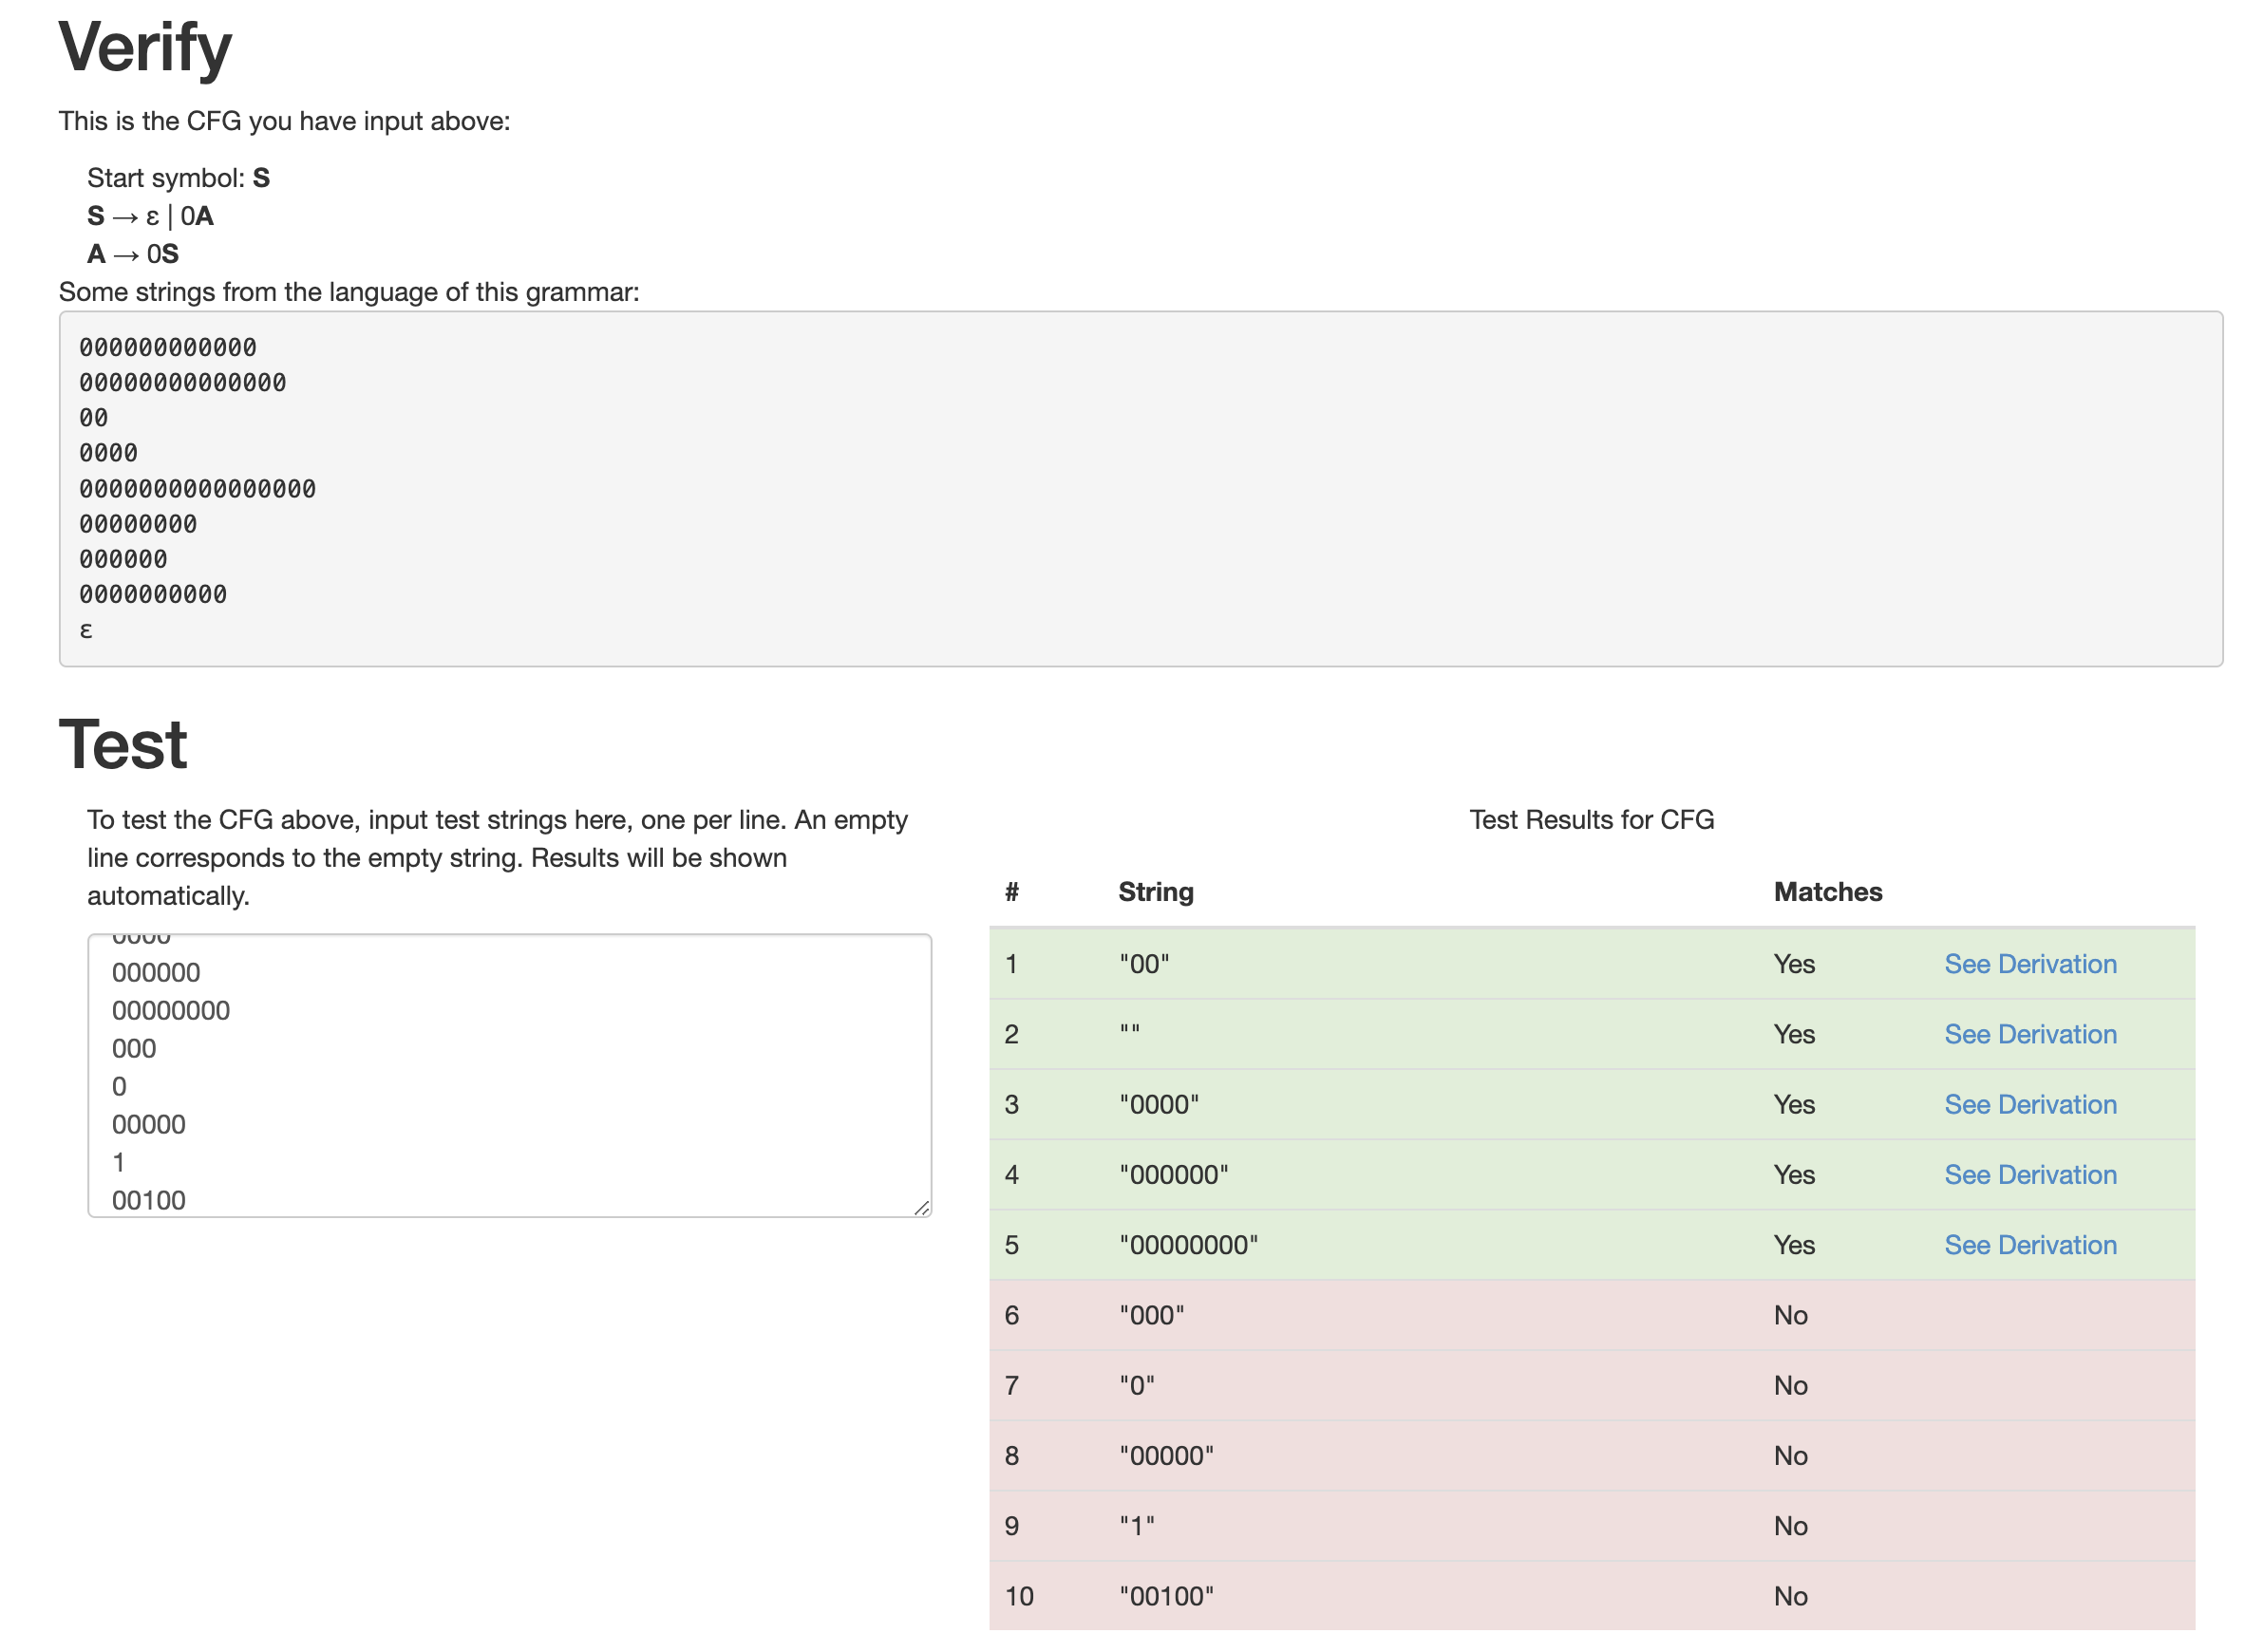
\includegraphics[width=0.9\linewidth]{hw8ss1.png}
    \caption{Screenshot of online tool tests.}
    \label{screenshot}
\end{figure}
\subsection*{Answer 2:}
\begin{figure}[htbp!]
    \centering
    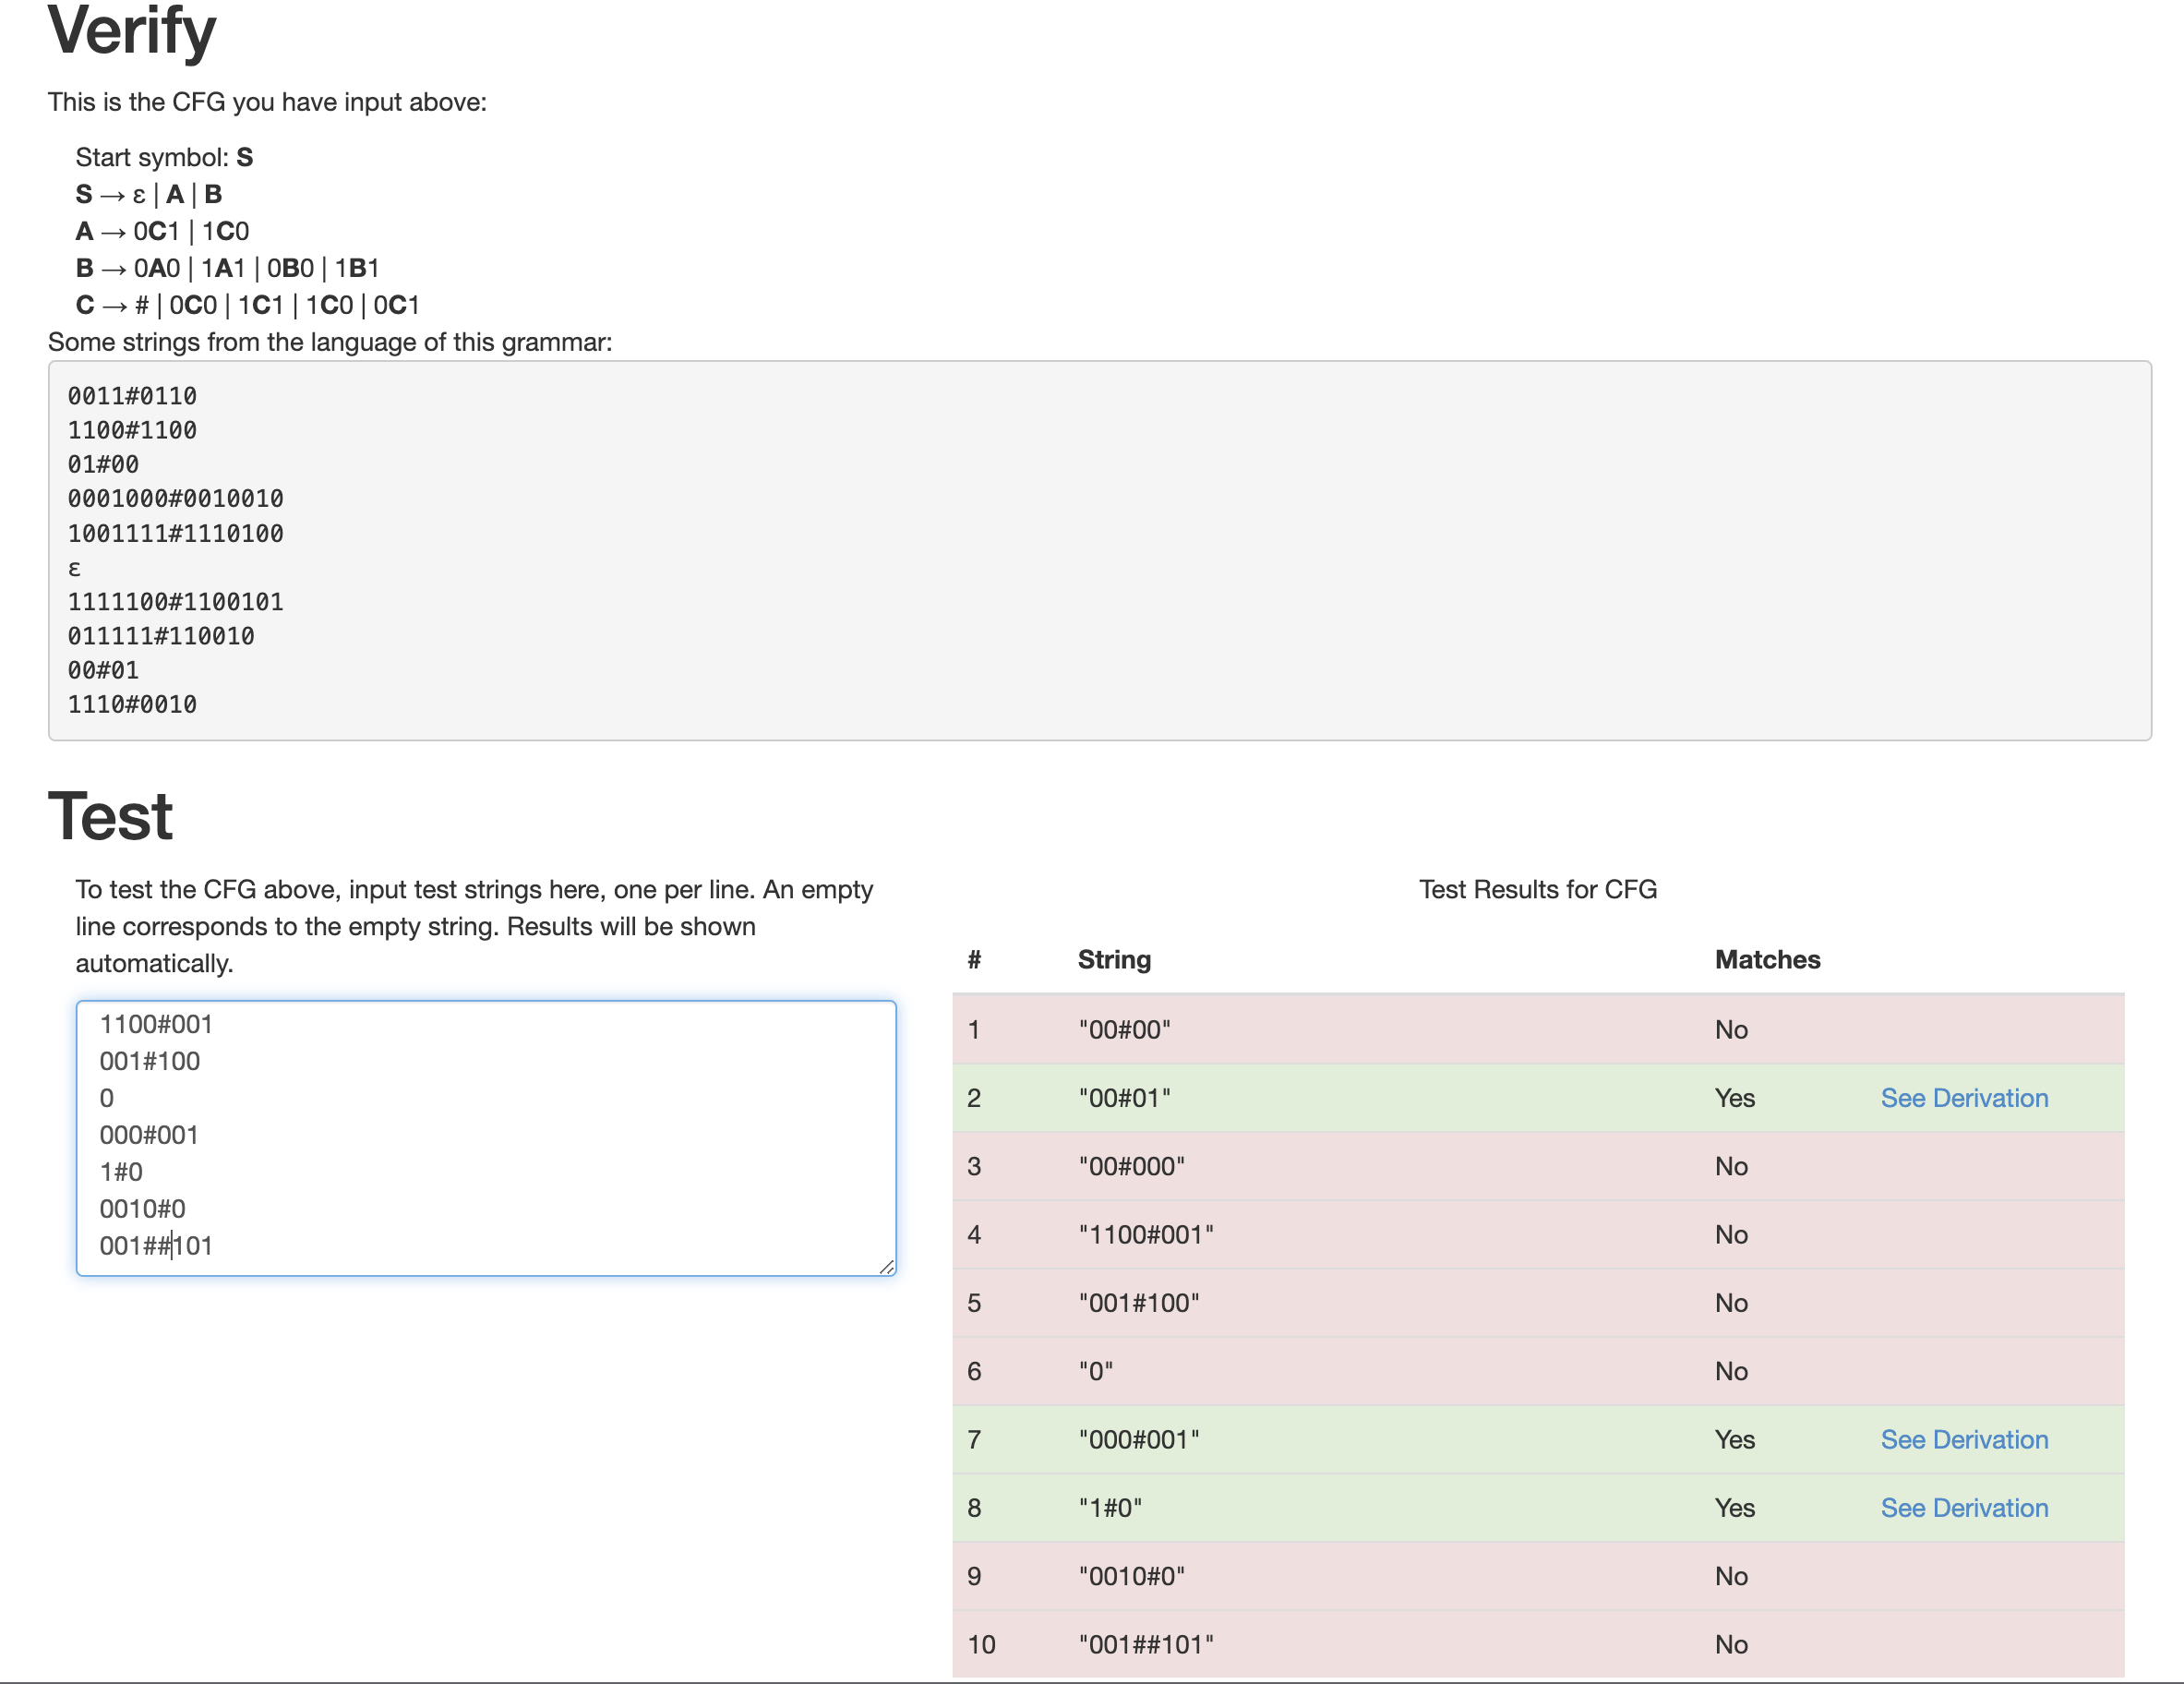
\includegraphics[width=0.9\linewidth]{hw8ss2.png}
    \caption{Screenshot of online tool tests.}
    \label{screenshot}
\end{figure}
\subsection*{Answer 3:}
\begin{figure}[htbp!]
    \centering
    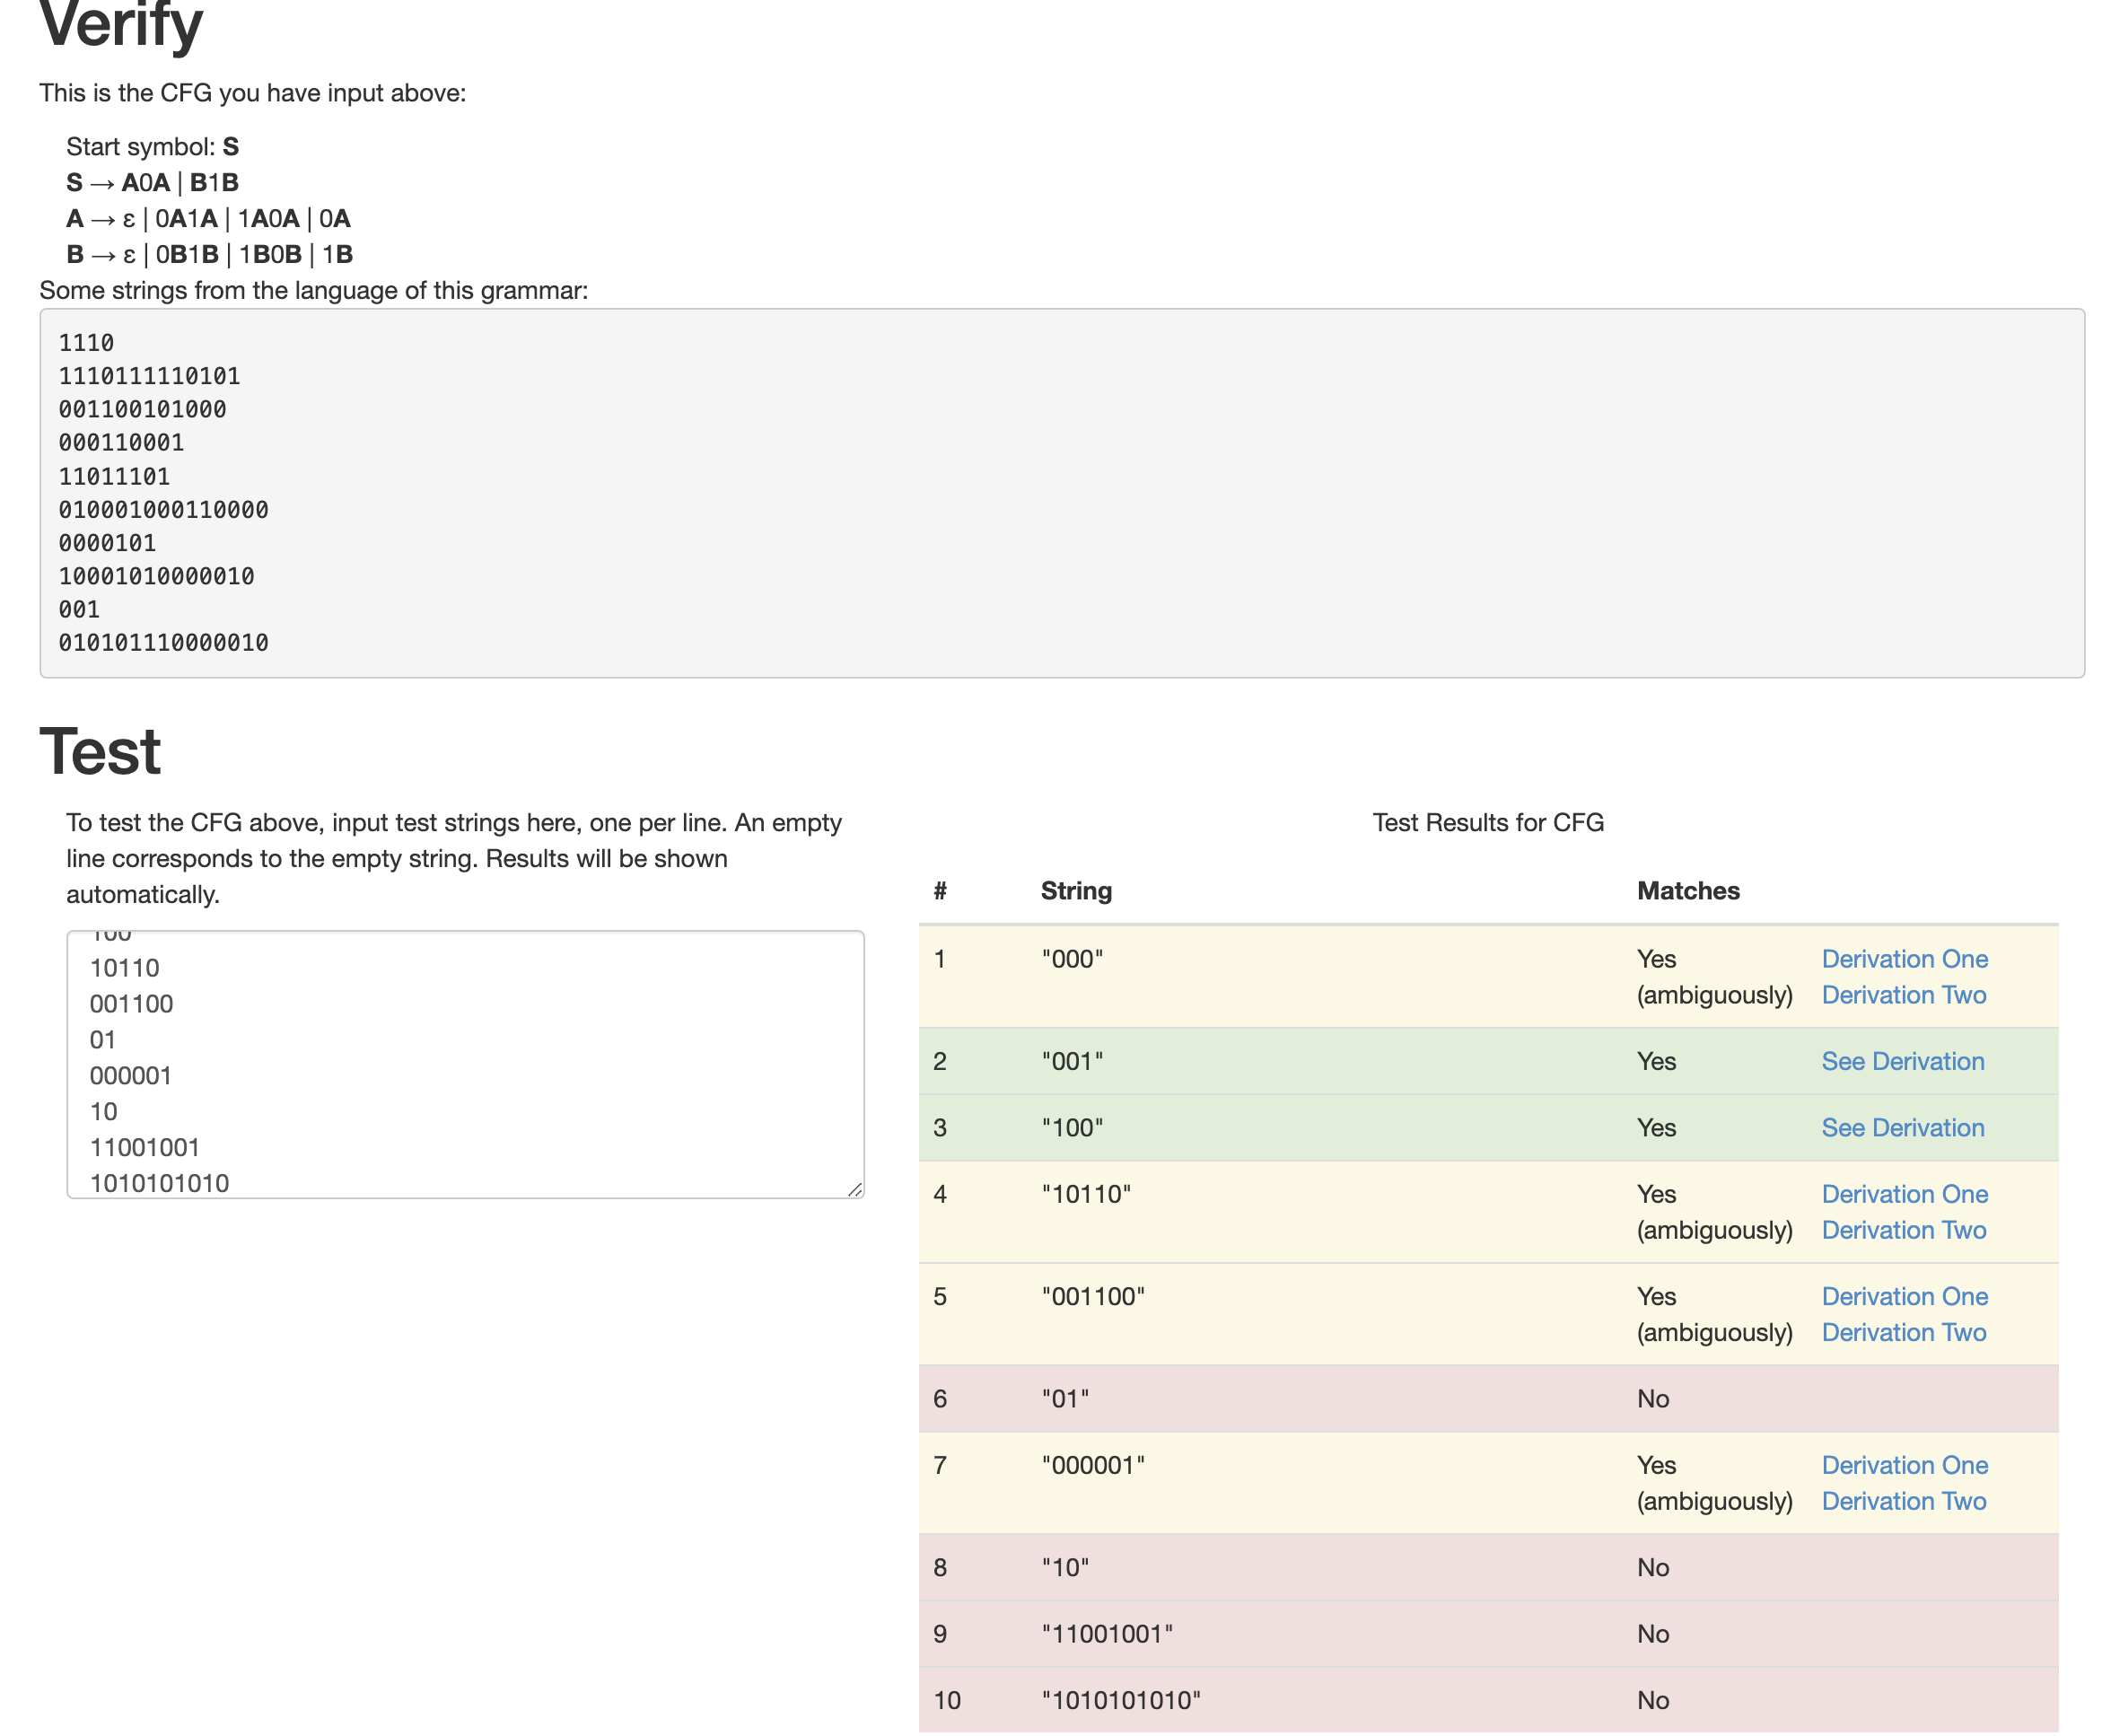
\includegraphics[width=0.9\linewidth]{hw8ss3.png}
    \caption{Screenshot of online tool tests.}
    \label{screenshot}
\end{figure}


\end{document}
